\subsection{Control Point Transfer}\label{sec:cp_transfer}
To transfer the extracted motion to the input sketch, we first need to map the control points specified on the video object to the sketch. This is done by aligning the sketch with the video. More specifically, we apply the Shape Context method~\cite{belongie2000shape} to build correspondence between the sketch image and the extracted object contour as described in Sec.~\ref{sec:motion_extraction}. For a control point inside the video object, we represent its location using barycentric coordinate of a set of evenly sampled contour points, and compute its location using the same barycentric coordinate on the sketch image. 
For sketches drawn over a keyframe using an over-painting interface similar to the EZ-Sketching system~\cite{EZSketching:2014}, the alignment step is optional, since the sketch is already well aligned with the underlying image.

%Thus the control points extracted from the video can be directly applied to drive the sketch animation. 
%


\subsection{Motion Transfer} \label{motion_transfer}

After tracking is done, we use the sparse control point trajectories to drive the final sketch animation. 
For this purpose, we first embed the sketch into a mesh and then use a mesh deformation method to warp the mesh for animation. The mesh is generated by
triangulating an expanded region of the sketch (see Fig. 1).
Our expectation for the deformation is twofold: 
(1) the deformed mesh should closely follow the guidance of the control points to preserve the extracted motion; 
and (2) the original sketch strokes should not be distorted too much to avoid unnatural deformation artifacts. 

Traditional controlled mesh deformation methods, like the as-rigid-as-possible (ARAP) mesh deformation \cite{Igarashi:2005}, are only designed to keep the rigidity of the mesh triangles (see Fig.\ref{fig:mesh}), but do not necessarily preserve the shape of the embedded strokes, 
especially for those crossing multiple triangles. In addition, in our preliminary study we have found that sometimes it is desirable to have parts of the sketch to be more rigid, while making other parts more flexible to capture large motion. 
Fig.~\ref{fig:deformation} shows such an example. 
Using the original ARAP deformation, the body of the bird is undesirably distorted by the large motion of its wings. 
In such a case, the user may want to apply a stronger rigidity constraint on the bird's body, while applying a weaker rigidity to its wings to better capture the intensive flapping motion.

To better attain user-specified local rigidity on the input strokes, 
we devise a variant of the ARAP method called {\em Stroke-preserving ARAP}. 
In order to preserve the stroke shape, our method adds new mesh triangles derived from the input strokes to the original  mesh. %\hongbo{the reviewer might ask what if you use constrained Delaunay triangulation. that is, the stroke points are used to constrain the triangulation?}
The original mesh is denoted as $ \mathcal{M}_0 = (\mathcal{V}_0, \mathcal{T}_0) $, as shown in gray in Fig.~\ref{fig:mesh}.
We uniformly sample points from each input stroke, and construct a \textit{sketch triangle} set $\mathcal{M}_s = (\mathcal{V}_s,\mathcal{T}_s) $ (purple triangles in Fig.~\ref{fig:mesh}), by connecting every three consecutive points on each stroke, excluding degenerate triangles on line segments. We then construct a \textit{link triangle} set $\mathcal{T}_l$, by connecting each vertex in $\mathcal{V}_s $ with the three vertices of the triangle in $\mathcal{V}_0$ on which it falls.

\begin{figure}
	\centering
	\includegraphics[width=0.85\linewidth]{images/mesh}
	\caption{The modified mesh used for stroke-preserving mesh deformation.}
	\label{fig:mesh}
\end{figure}


Given the augmented mesh structure $\mathcal{M}=(\mathcal{V}_0 \cup \mathcal{V}_s, \mathcal{T}_0\cup \mathcal{T}_s\cup \mathcal{T}_l)$, we formulate the stroke-preserving ARAP deformation as the following energy minimization problem: 
\begin{align}\label{eqn:deformationE}
	\min_\mathcal{M} \ E_0 + \beta E_{link} + \gamma E_{sketch},
\end{align}
where $ E_0 $ is the deformation energy of the original mesh $ \mathcal{M}_0 $; $ E_{link} $ and $ E_{sketch} $ are the deformation energy terms of the newly constructed triangle sets $\mathcal{T}_l $ and $\mathcal{T}_s $, respectively. 
Specifically, following \cite{Igarashi:2005}), for each triangle set, we have:
\begin{align}
 E(\mathcal{T}) = \sum_{t\in \mathcal{T}} \sum_{v_i, v_j \in t} \|\overrightarrow{v'_iv'_j} - H\overrightarrow{v_iv_j}\|^2 ,
 \end{align}
  where $ H $ is a rigid transformation matrix that is achieved by a two-step optimization algorithm; please refer to \cite{Igarashi:2005} for more details.
The same definition of $E(\mathcal{T})$ is applied to $\mathcal{T}_0, \mathcal{T}_{link}, \mathcal{T}_{sketch}$.
 Minimizing $ E_{sketch} $ keeps the shape of the strokes while minimizing $ E_{link} $ transfers the deformation of the original mesh to the strokes. 
In our system, we set the weight $ \beta $ to be a small value of 0.01, as we allow the triangles in the link triangle set to be distorted to balance between deformation and sketch shape preserving. We set $ \gamma = 1$ by default in order to better preserve the sketch shape. 
For all the strokes that need to be more rigid, we increase the corresponding $\gamma$ value by a factor greater than one. The local rigidity brush is also accumulative so the more the user brushes, the more rigid that the underlying sketch strokes will be. 

%{\bf User-specified local rigidity.} 
%The energy defined in Equation~\ref{eqn:deformationE} applies the same shape preserving weight $\gamma$ to all sketch strokes.


%\Jue{An example is shown in the accompanying video.}

\begin{figure}
	\centering
	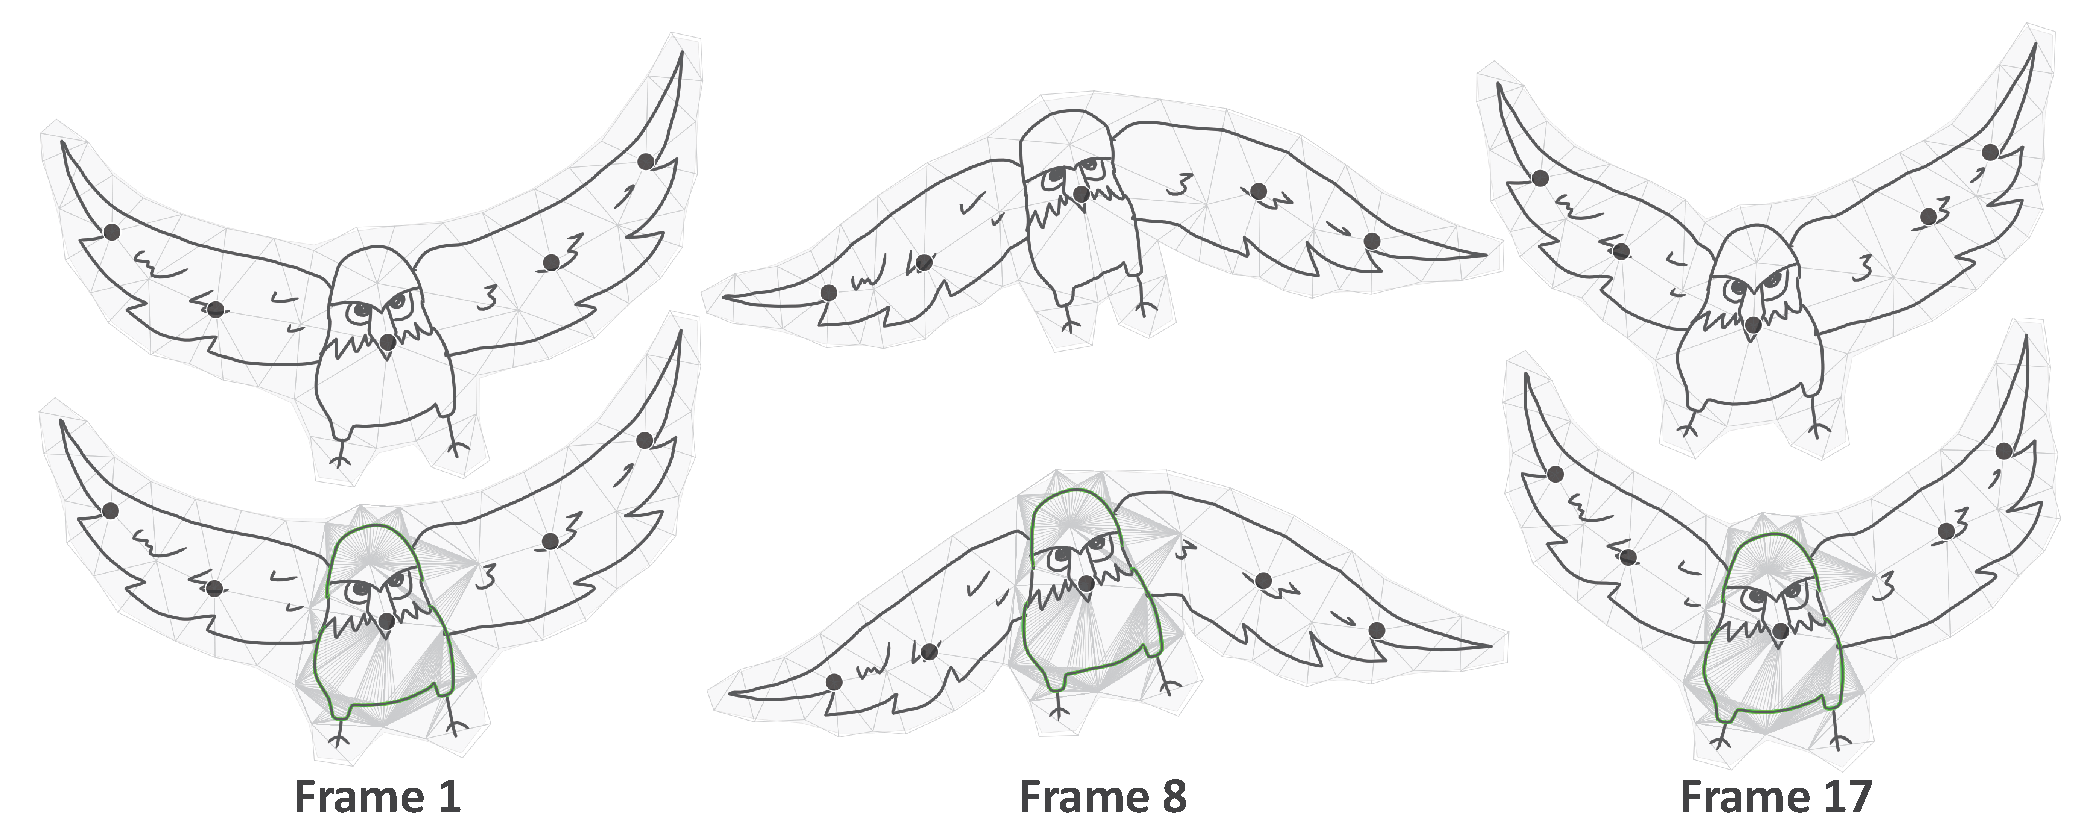
\includegraphics[width=\linewidth]{images/deformation}
	\caption{Sketch deformation results with (bottom) and without (top) applying the shape preserving method described in Sec.~\ref{motion_transfer}. The stroke in green is set to be more rigid.}
	\label{fig:deformation}
\end{figure}

\if 0
\subsection{Extensions}

\sout{
To reuse the extracted motion, we also extend it for sketches that are not similar to video objects. The main goal is to map the original key points of the video to the new sketch. This could be solved by finding the matching between the original sketch and the new one. 
We first obtain the sketch contours, $ s_o, s_n $, of the original and new sketches using the method in \ref{motion_extraction}. Then we sample $ k_0 $ and $ k_n $  points, $ \textbf{P} = \{p_i\} $ and $ \textbf{Q} = \{q_i\} $, inner the two contours. Then the correspondence could be obtained by finding the affine transformation $ T $ between the two point sets by ICP point matching methods. Then for any point $ x_o $ inner $ s_o $, we could find the corresponding position $ x_n $ inner $ s_n $ by   Given a key point's position of the first frame, $ x_i $, we first compute $ k $ nearest points in $ P $ and its corresponding points in $ \textbf{Q} $. Then the corresponding position $ x_n $ could be computed by the berry centric weight of the $ k $ points of $ \textbf{Q} $. If $ x_n $ is located outside of $ s_n $, then we remove one point from the $ k $ points and re-compute the position until $ x_n $ is located inside of $ s_n $. }
\fi

\subsection{Multiple-Layer Animation}\label{sec:multi-layer_animation}

As discussed earlier, single layer, mesh-deformation-based animation cannot handle topology change, which is common for dynamic objects (see Fig.~\ref{fig:multilayer}a). 
To handle such cases, our system allows the user to create animations with multiple layers. 
Using this tool, the user first divides the sketch strokes into several groups, each representing a layer (Fig.~\ref{fig:multilayer}b).
To avoid detaching different layers from each other in the animation, our system then automatically detects the intersections of these layers, and adds one {\em joint point} at the center of each intersection region (Fig.~\ref{fig:multilayer}c, blue circles). 
%The system then moves layers in each animation frame to make sure that the layers still attach at the joint points. 
%Our system automatically adds a joint for any two partially-overlapping layers, which is the center of the overlapping area. 
During the motion transfer stage, we first deform each layer individually based on their control points, and then re-connect meshes of layers based on the joints, as shown in Fig.~\ref{fig:multilayer}d-e. 
\begin{figure*}
	\centering
	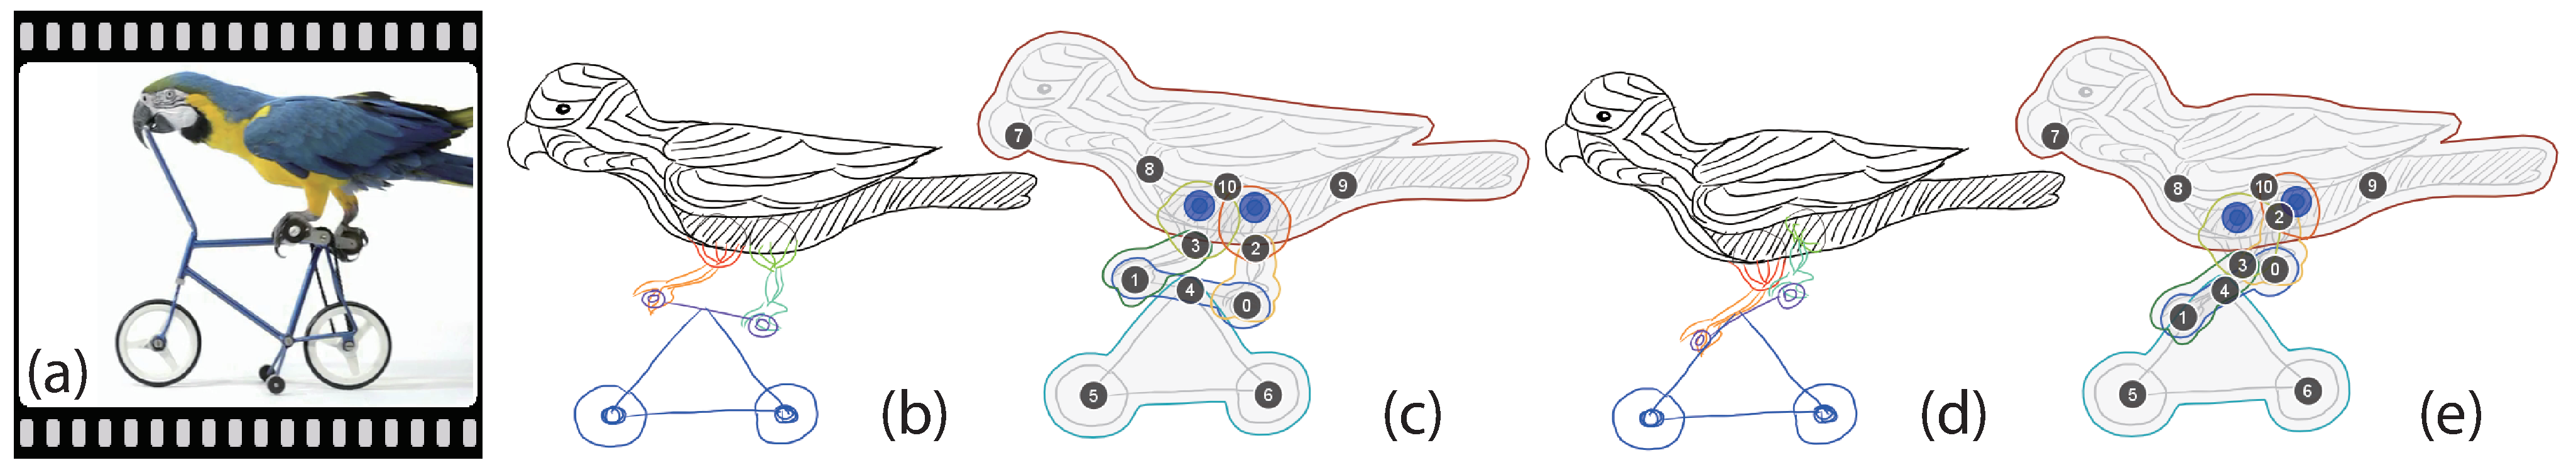
\includegraphics[width=\linewidth]{images/multilayer2}
	\caption{Multiple layer animation to handle self-occlusion and topology change. When the two legs of the macaw cross, they  introduce severe occlusion and topology change that cannot be handled by a single mesh layer. Our system allows the user to decompose the mesh into multiple layers (shown in different colors) to properly handle it. (a) Input video. (b) Grouping strokes into layers, visualized in different colors. (c) Control points and layer joints (blue circles). (d-e) Deformed sketch and new point layout in another frame.}
	\label{fig:multilayer}
\end{figure*}

%Our system aims at providing the user with an easy way to add 3D strokes to an existing shape for communicating conceptual design ideas. Strokes drawn by a user over an existing 3D shape are generally of two types. The first type lie on an existing surface. The 3D information for such a stroke can be determined easily by projection onto the surface. The second type of strokes are drawn to specify a non-existent part of the shape, indicating how the original shape is to be modified. Determining the 3D information for this type of stroke is nontrivial. Our system focuses on providing an interface to draw sketch strokes of the second type.

%We will conduct a user study to evaluate our system. The user study will consist of two parts. In User Study I, a number of participants will be invited to use both our system and an existing state-of-the-art keyframe method such as Adobe Animator to create two animations for every given pair of sketch and video. 
%To evaluate the efficiency of our system, 
%%In this experiment, the participants will be asked to create a sketch animation to a given video. 
%we will compare the completion time and the number of operations which include the sketching operations and the editing operations. 
%The participants will also be asked to answer a questionaire on the usability of our system. 
%
%The sketch animations created using the two methods will then be evaluated by a different group of participants in User Study II.
%We will ask the participants to score each sketch animation created in User Study I on aesthetics, completeness, etc. 


%\begin{figure}
%	\centering
%	\includegraphics[width=0.9\linewidth]{images/trackingcomparison}
%	\caption{}
%	\label{fig:trackingcomparison}
%\end{figure}

% Please add the following required packages to your document preamble:
% \usepackage{multirow}
%\begin{table*}[]
%	\centering
%	\caption{My caption}
%	\label{my-label}
%	\begin{tabular}{l|cc|cc|cc|cc|cc}
%		\hline
%		\multirow{2}{*}{} & \multicolumn{2}{c|}{\textbf{OURS}} & \multicolumn{2}{c|}{\textbf{STRUCK}} & \multicolumn{2}{c|}{\textbf{SPOT}} & \multicolumn{2}{c|}{\textbf{SAMF}} & \multicolumn{2}{c}{\textbf{DT}} \\
%		& \textit{Err.}    & \textit{Pre.}   & \textit{Err.}     & \textit{Pre.}    & \textit{Err.}    & \textit{Pre.}   & \textit{Err.}    & \textit{Pre.}   & \textit{Err.}  & \textit{Pre.}  \\ 
%		\textbf{Candle}   & 0.999            & 0.982           & 36.451            & 0.675            & 13.439           & 0.786           & 28.552           & 0.737           & 35.962         & 0.615          \\
%		\textbf{Cartoon}  & 1.806            & 0.940           & 3.731             & 0.884            & 7.206            & 0.759           & 5.217            & 0.801           & 7.397          & 0.744          \\
%		\textbf{Fish}     & 3.537            & 0.820           & 13.600            & 0.587            & 25.516           & 0.179           & 43.196           & 0.434           & 43.525         & 0.345          \\
%		\textbf{Kangaroo} & 4.574            & 0.805           & 12.598            & 0.666            & 19.727           & 0.427           & 44.419           & 0.282           & 21.830         & 0.415          \\
%		\textbf{Kite}     & 6.534            & 0.727           & 21.293            & 0.465            & 9.435            & 0.618           & 13.159           & 0.663           & 28.399         & 0.404          \\ \hline
%	\end{tabular}
%\end{table*}
%\qingkun{To-Do}
%We will extend the basic \textit{Live Sketch} to two applications.
%%	\textbf{Many-to-one motion transfer}
%Segmenting a character into meaningful parts or layers and animating them separately is common in animation creation. Similarly, our system will also allow transferring motions from multiple videos to different parts of a single sketch. Independent motion transfer for each part will lead to spatial inconsistency, which can be solved by existing motion retargeting method such as AniMesh~\cite{Jin:2015}.
%Another way to increase the usability of motions is to transfer motions to a sketch in different temporal intervals.  We will need to address the issue of smooth transitions between motions.
%Note that in such scenarios the number of control points used in the two motions may be different but the original mesh is the same as
%the two motions are transferred to the same sketch. 
%%the two sets of control points positions between the two control point sets at the transition position may not be well aligned and may locate at different parts of the sketch. 
%A possible solution to attain smooth transition from motion A to motion B is as follows (see Figure 6). We first compute the position of each control point of A on B's deformed mesh by mesh interpolation. Next we can find a new motion trajectory for each point of motion A during B's time interval. A smooth transition trajectory can easily be found between the two trajectories by Hermite 
%interpolation.
%by Laplacian smoothing after connecting them. 
%Similarly, we can obtain a smooth transition trajectory for each control point of motion B. Therefore, the animation can be transited smoothly based on the transition trajectories.

%Interactive illustrations can provide a more playful or informative experience~\cite{Kazi:2014b}. We will also extend our \textit{Live Sketch} tool to achieve dynamic interactive animations. Users can interact with the animation to control its playback direction, speed of playing and locally deform near a dragged point. 
%We will provide a user interface that when the user drags one part of the sketch, the animation will be played forward or backward according to the drag direction with respect to the nearest motion trajectory. The speed of playing will depends on the cursor speed.  The point on the sketch where it is being dragged will be deformed such that it stays attached to the cursor. This can be achieved by applying a sketch deformation method described in Task D, where the drag point is treated as an additional control point.
%% (user is also required to give another static point). 
%Different dynamic motion constraints can also be specified to different parts, for example, producing the effect of magnifying the motion of certain parts while suppressing the motion of the other parts. 
%Furthermore, dynamic dragging constraints can also be applied to simulate effects such as flowers being blown by wind.  

%It also allow user to add an external force like wind with dynamic direction and speed.
%We provide a user interface that when user drag some part of the sketch, the animation would be played adaptively and dynamically and also respect to user's dragging position. The animation speed and direction can be computed by the dragging speed and direction. To make sure that the dragging part is always attached to the cursor, a sketch deformation is applied to the deformed sketch using the method in Task D, where the dragging point is treated as the control point (user is also required to give another static point). Furthermore, our system can also produce dynamic animation when user specifies dynamic dragging constraints such as the wind, or highlights the motion of some parts by magnifying its motion and reducing others'.

%
%\subsection{Extensions}
%
%Our tool aims to animate a sketch using the same motion of the object in the video, it thus will look as real as in the video. Since the users might want to produce a stylized animation, we will provide post-animation stylization tools, such as using animation filters~\cite{Wang:2006}, applying the 12 animation principles~\cite{Kazi:2016}, and adding animation looping.
%
%%{The methodology described above focuses on motion transfer for a single object.} An extracted motion can also be re-used and transferred to multiple objects.  In that case, motion re-targetting is necessary. 
%
%%We will also investigate creation of sketch animations containing numerous objects. For this purpose, we will need to design and implement a new user interface that can combine the results of several animation results of our method into one scene.
%
%Sketching on touch-based devices is direct and natural. Hence,
%implementing Live Sketch on devices like iPad and iPhone will be highly desirable.  This will require redesigning the user interface to improve user experience on sketching and interactions, such as integrating multitouch features and stylus pen.

%In our system, we require only coplanar strokes be drawn in each step. This setting ensures that our system is able to generate the expected 3D sketch with only simple interaction. However, this restriction may hinder the user during drawing. The ultimate goal of allowing the user to draw strokes on arbitrary planes or surfaces in any order is too difficult. Instead, we will further investigate how to make our system more general by introducing other type of constraints besides the coplanar constraint for drawing strokes, constraining the current set of drawn curves to be on a curved surface, or to be symmetric. 
%%\ca{Similar to the current algorithm, we will borrow the geometry information to constrain the drawn curves. Specifically, 
%If the matched sharp edges are on a common curved surface that is extracted from the shape, the surface is a potential canvas. If the drawn strokes are self-symmetrical after an affine transformation, the canvases that realize this transformation might be desirable ones. When the user draws a set of strokes, it is unknown which constraint should be used. A possible solution will be to traverse all the constraints and generate all possible candidate 3D strokes which will be ranked using the same criteria described before.

%An issue to solve then would be how does the system automatically recognize what type of constraint to enforce on the drawn strokes. \ca{Possible solutions? curved surface derived from the given shape}

%Man-made shape is the main focus of our system. It is because designing man-made shapes is more common than organic shapes. 
%For example, the user may want to modify the design of an existing furniture model, or change the appearance of a building model. When designing a 3D scene, the models in this scene are mostly man-made. In our system, we will mainly focus on the following information.




%\section{Methodology}
%The pipeline of our system is shown in Fig~\ref{overview}. Given two inputs sketch and the video, our method contains three main steps to animate the static sketch $ \mathcal{S} $:
%
%\begin{description}
%	\item[Video\&Sketch Alignment.] Alignment between the sketch (vector graphics) and video frame (bitmap image) is very hard. We proposed a method that extracts the feature points both good to track in video and in the region of user's interest in sketch.
%	\item[Motion Extraction.] Drifting problem is always hard to avoid in video tracking, which could produce unexpected animation results. We present a   tracking method that keeps the object structure even when some parts drifts at some frames.
%	\item[Motion Transfer.] With the correspondence and the extracted video motion, we animate the sketch using a stroke-preserving as-rigid-as possible mesh deformation method. This method could keep the stroke shape well even with large deformation. 
%\end{description}
%
%\begin{figure*}[t]
%	\centering
%	\includegraphics[width = 0.95\linewidth]{images/overview}
%	\caption{Given the sketch and the video, the first step alignment would try to extract some good feature points from video and sketch and compute their correspondence.
%		Then we extract the motion by tracking the good feature points of the video by using object structure.		
%		Combined with the correspondence and the motion, we used a stroke-preserving ARAP method to transfer the motion to the sketch.
%		After the three steps, the final sketch animation is generated. 
%	}
%	
%	\label{fig:overview}	
%\end{figure*}
%
%\subsection{Video\&Sketch Alignment}\label{alignment}
%Finding the correspondence between video and sketch is tough problem, because the latter is more abstract and semantic. Therefore, we need to extract the feature points that are both good to track for video and good to control for sketch.
%
%We first extract the good feature to control for sketch and to track of the first video frame by scale irrelevant corner detection method[XXX]. Then a graph matching is used to find the best one-to-one mapping between the two feature point set [XXX].
%
%However, sometimes it would be hard or even impossible to detect the correspondence, because the sketch and the video object do not have similar structure (see the example in Fig. [XXX]). we also provide a user interface to edit the flexible correspondence. 
%
%\begin{figure}
%	\centering
%	\includegraphics[width=0.85\linewidth]{C:/Users/suqin/Documents/flexible}
%	\caption{}
%	\label{fig:flexible}
%\end{figure}
%
%
%\subsection{Motion Extraction}\label{motion_extraction}
%The goal of this step is extract robust motion for each feature point that is extracted in previous step. We proposed a method that could 
%1)track the object that could preserve its structure 2) keep the structure by using the structure even if drifting problem happens at some parts.
%Unlike previous graph-based or structure-preserving object tracking methods, our method could detect the drifting parts and predict its positions by spatial and temporal neighborhood.
%Our structure preserved object tracking method mainly considers two part: 1) $ E_t $ appearance energy that existing tracking methods 2) $ E_s $structure energy that measures the structure deformation. Assuming that we could obtain several candidates for the $ i $th part, $ \{ c_{ij} \} $ ($ c_{ij} $ is contains the candidate position $ p_{ij} $ and same size with initial frame), with appearance energy ascending order. So this could be formulated as a energy minimization problem
%\[ E* = \min_{C \in \mathcal{C}} E_t(C) + \alpha E_s(C) \]
%over all candidate configurations in $ \mathcal{C} $, where $ E_s = \sum_{e} \Delta d + w\sum_{\theta} \Delta \theta$ is measured by the edge length and angle difference regarding to initial object position.
%
%However, 1) it requires searching exponentially many configurations; 2) some candidates may break the structure even if they may have small appearance energy. To solve this problem, we will propose a method that could detect the bad candidates, preserve the global structure by the good ones and then predict the positions by its spatial and temporal neighborhood.
%
%%\begin{algorithm}
%%	\caption{Motion Extraction}\label{euclid}
%%	\begin{algorithmic}[1]
%%		\Procedure{MyProcedure}{}
%%		\State Initialize: $ C^* \gets (c_{11}, c_{21}, ..., c_{i1}, c_{n1}) $
%%		
%%		
%%		\While {true}
%%		\State $ i^* \gets \max_i E_t(C^*_i) + \alpha E_s(C^*-C^*_i) $
%%		\State $ j^* \gets \min_j E_t(c_{i^*j}) + \alpha E_s(C^*-C^*_{i^*} + c_{i^*j}) $
%%		
%%		\EndWhile
%%		
%%		\State $\textit{stringlen} \gets \text{length of }\textit{string}$
%%		\State $i \gets \textit{patlen}$
%%		\If {$i > \textit{stringlen}$} \Return false
%%		\EndIf
%%		\State $j \gets \textit{patlen}$
%%		\If {$\textit{string}(i) = \textit{path}(j)$}
%%		\State $j \gets j-1$.
%%		\State $i \gets i-1$.
%%		\State \textbf{goto} \emph{loop}.
%%		\State \textbf{close};
%%		\EndIf
%%		\State $i \gets i+\max(\textit{delta}_1(\textit{string}(i)),\textit{delta}_2(j))$.
%%		\State \textbf{goto} \emph{top}.
%%		\State \Return $ C $
%%		\EndProcedure
%%		
%%	\end{algorithmic}
%%\end{algorithm}
%
%\subsection{Motion Transfer}\label{motion_transfer}
%
%Motion transfer aims to transfer the extracted motion of video to the sketch by using the extracted correspondence in section \ref{motion_extraction}. The simplest way is using as-rigid-as possible(ARAP) mesh deformation method.
%To generate the mesh that is used to deform the sketch, we triangulate the contour that is obtained by active contour method for the sketch image. Then we can animate the sketch by deforming the mesh with the feature points' position as handles. However, ARAP mesh deformation could not preserve the stroke shape because it only keeps the rigidibility of the mesh triangles (see the example in Fig.XXX). 
%
%Therefore, we proposed stroke-preserving ARAP method to preserve the stroke shape during the mesh deformation.
%Denote the feature positions of the $ t $th and $ (t + 1) $th frame as $ \mathbf{p}^t = \{p^t_{i}\} $ and $ \mathbf{p}^{t+1} = \{p^{t + 1}_{i}\} $.
%To preserve the stroke shape, we reconstruct the original mesh $ \mathcal{M}_0 = (\mathcal{V}_0, \mathcal{T}_0) $ by adding one vertex set $ \mathcal{V}_s $ that includes all the sketch points and two triangle sets $ \mathcal{T}_s, \mathcal{T}_l $, where
%
%\begin{description}
%	\item[Sketch triangle set $\mathcal{T}_s $] is constructed by connecting every three consequent points on each stroke;
%	\item[Link triangle set $\mathcal{T}_l $] is constructed by connecting each sketch point with its outer triangle�s vertices.
%\end{description}
%
%\begin{figure}[t]
%	\centering
%	\includegraphics[width = 0.95\linewidth]{images/mesh}
%	\caption{Reconstructed mesh for stroke-preserving ARAP deformation.}
%	
%	\label{fig:mesh}	
%\end{figure}
%
%Then, the ARAP mesh deformation is applied to the new constructed mesh $ \mathcal{M} = (\mathcal{V}, \mathcal{E}) $ where $ \mathcal{V} = \mathcal{V}_0 \cup \mathcal{V}_s $ and $ \mathcal{E} = \mathcal{E}_0 \cup \{e|e\in \mathcal{T}_s \cup \mathcal{T}_l\} $ by the following energy minimization formulation:
%\[ \min E_0 + E_{1ink} + \beta E_{sketch} \]
%, where $ E_0 $ is deformation error of the original mesh $ M_0 $, $ E_{1ink} $ and $ \beta E_{sketch} $ represents the error of the new added triangle sets $\mathcal{T}_s $ and $\mathcal{T}_l $. The main idea of this method is that the original mesh will try to deform the sketch triangles through the intermediate link triangles. If the weight of the stroke triangles are large enough, the shape of the stroke would be preserved. $ \beta $ is set to be 10 in our implementation.
